\chapter{Тестирование приложения} \label{chapt4}

По итогам разработки производятся тестовые испытания, позволяющие установить корректность функционирования разработанного программного комплекса и проверить соответствие функциональным требованиям. Логически, проект делится на серверную и клиентскую части. Основная задача серверной части - обработка сообщений и событий, приходящих от браузера, клиента. Самая сложная, нестабильная и слабопереносимая(между операционными системами) часть функциональности сервера состоит в автоматизации работы с программами RTKLIB. Именно этот модуль показал наименьшую стабильность при разработке и долговременном использовании. Дело в том, что ошибки при парсинге вывода этих программ, особенно управляемых интерактивной консолью, могут проявлять себя не сразу. Кроме того, данные модули являются критическими для приложения, ведь они предоставляются всю основную информацию, нужную для интерфейса. Таким образом, было решено создать модульные тесты для классов, управляющих работой RTKRCV, STR2STR и CONVBIN. Это позволило упростить разработку и дополнение этих классов новой функциональностью, без риска внести новые ошибки в код. Тестирование приложения можно разделить на две части:

\begin{enumerate}
  \item Тестирование модуля, отвечающего за работу с RTKLIB;
  \item Тестирование функциональности интерфейса;
\end{enumerate}

\section{Модульное тестирование классов, работающих с RTKLIB} \label{sect4_1}

Работа с модульными тестами будет рассмотрена на примере класса RtkController, автоматизирующего работу с RTKRCV. В качестве фрэймворка для юнит-тестирования был выбран стандартный для Python \textbf{unittest}.

Для создания тест-кейса при работе с unittest, требуется отдельный файл, описывающий сценарий нового теста. Тест в данном файле принимает форму класса, унаследованного от класса \textbf{unittest.TestCase}.

\lstinputlisting[
  label={listings:RtkController_test},
  caption={Класс RtkControllerTest},
  style={java}
]
{src/RtkController_test.py}

Методы данного класса представляют собой отдельные тесты. Также есть специальные методы, унаследованные от класса-родителя - \textbf{setUp} и \textbf{tearDown}. Эти методы следует переопределить, так как они вызываются при каждом из определенных пользователем тестов. В случае тестирования RtkController, setUp и tearDown переопределены для создания объекта класса RtkController и запуска RTKRCV до теста, а также остановки приложения после его выполнения. Такая структура класса позволит отделить запуск и остановку программы от функционального теста, проверяющего, например, получение корректного статуса, и таким образом получить более точные диагностические данные.

Перед каждым тестом, описанным ниже, вызывается RtkController.setUp(). Происходит проверка корректного запуска Rtkrcv с помощью метода \textbf{assertTrue}. Возврат значения False, а также любое брошенное исключение будет означать провал теста еще на этапе setUp.

\lstinputlisting[
  label={listings:RtkController_setUp},
  caption={Метод setUp класса RtkControllerTest},
  style={java}
]
{src/RtkController_setUp.py}

После успешного выполнения теста вызывается RtkController.tearDown(). После остановки RTKRCV, происходит проверка корректного завершения программы.

\lstinputlisting[
  label={listings:RtkController_tearDown},
  caption={Метод tearDown класса RtkControllerTest},
  style={java}
]
{src/RtkController_tearDown.py}

Тесты функциональности класса RtkController состоят в вызове других методов класса RtkController, например getStatus(). Этот метод сравнивает полученный объекта статуса с перечнем нужных параметров, которые выводит RTKRCV, чтобы проверить правильность парсинга вывода. Также, это происходит несколько раз подряд, для проверки надежности эмуляции консоли.

\lstinputlisting[
  label={listings:RtkController_testStatus},
  caption={Метод testStatus класса RtkControllerTest},
  style={java}
]
{src/RtkController_testStatus.py}

По такому же приниципу устроен тест метода getObs(). Однако, команда \textbf{obs} не возвращает информацию о спутниках при отключенной антенне, а значит достаточно получения пустого словаря и отсутствия брошенных исключений.

\lstinputlisting[
  label={listings:RtkController_testObs},
  caption={Метод testObs класса RtkControllerTest},
  style={java}
]
{src/RtkController_testObs.py}

\section{Функциональное тестирование интерфейса} \label{sect4_2}

Для данного прилоежния, тестирование интерфейса является тестированием на уровне приложения. Именно здесь проверяется корректность работы основых функций приложения - отображение статуса и настроек в режиме ровера, отображение настроек в режиме базы и отображение доступных логов спутниковых данных. В системе есть две возможности посмотреть логи приложения. В GNU/Linux, с помощью утилиты \textbf{journalctl} в составе \textbf{systemd} можно просматривать логи серверной части приложения. Для клиентской части приложения, в составе инструментов разработчика любого современного браузера, существует Javascript консоль. Контроль отсутствия ошибок в этих логах двух частей приложения и получение ожидаемых результатов работы гарантируют успешность тестов и корректность работы прилоежния. Для тестирования интерфейса были разработаны несколько методик, позволяющие проверить основные функции, выполняемые этим интерфейсом:

\begin{enumerate}
  \item Запуск приложения и состояние всех вкладок веб-страницы;
  \item Запуск режима ровера и получение корректного статуса, включая уровни спутников на графике;
  \item Изменение настроек RTKRCV и проверка, что эти изменения вступили в действие;
  \item Запуск режима базы и проверка получения поправок;
  \item Проверка возможности скачать лог в формате RINEX из списка логов;
\end{enumerate}

%%%%%%%%%%%%%%%% UI testing cases

\subsection{Тестирование запуска и загрузки приложения} \label{subsect4_2_1}

\underline{Исходные данные.} Приложение не запущено.

\underline{Ожидаемый результат.} Доступна страница , состоящая из четырех вкладок: \textbf{Status}, \textbf{Config}, \textbf{Logs} и \textbf{Settings}. Состояние по умолчанию - незапущенный ровер. В логах, доступных при помощи \textbf{journalctl} отсутствуют ошибки.

\underline{Последовательность действий:}

\begin{enumerate}
  \item Запустить файл \textbf{server.py};
  \item После сообщения о готовности сервера, перейти на нужный IP адрес с помощью браузера;
\end{enumerate}

\underline{Результат.} Совпал с ожидаемым. На группе рисунков 4.1 представлены вкладки описанной выше страницы при открытии в браузере смартфона.

\begin{figure}
  \label{img:latex}
  \begin{subfigure}{\linewidth}
    \center
    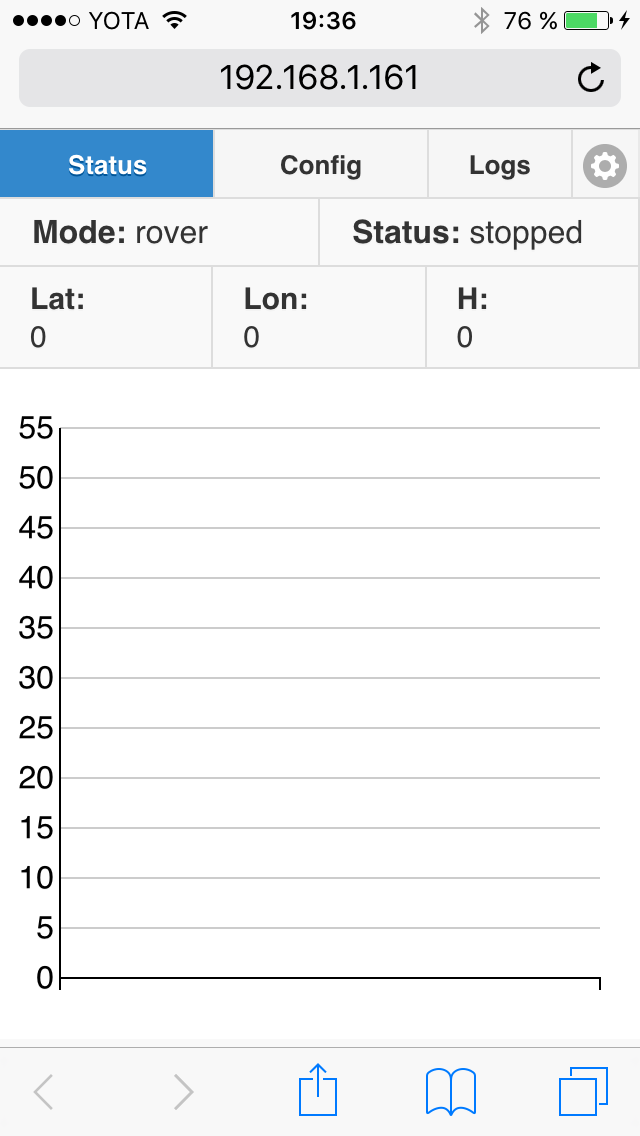
\includegraphics[width=.35\linewidth]{ui_testing_status_tab}
    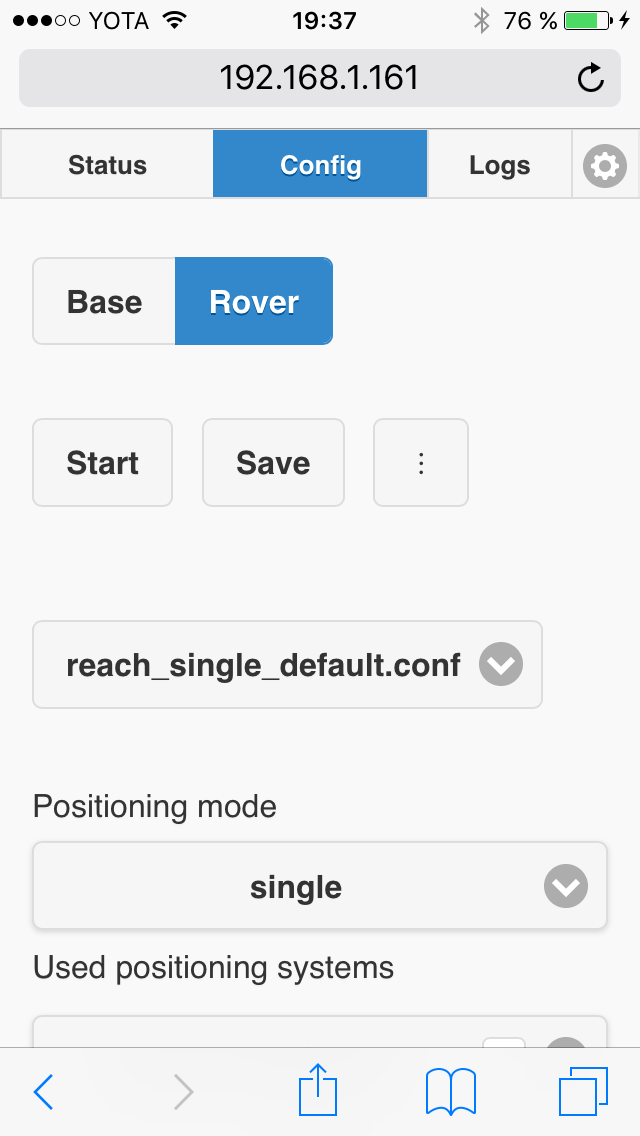
\includegraphics[width=.35\linewidth]{ui_testing_config_tab}
    \caption{Status и Config}
  \end{subfigure}\par\medskip
  \begin{subfigure}{\linewidth}
    \center
    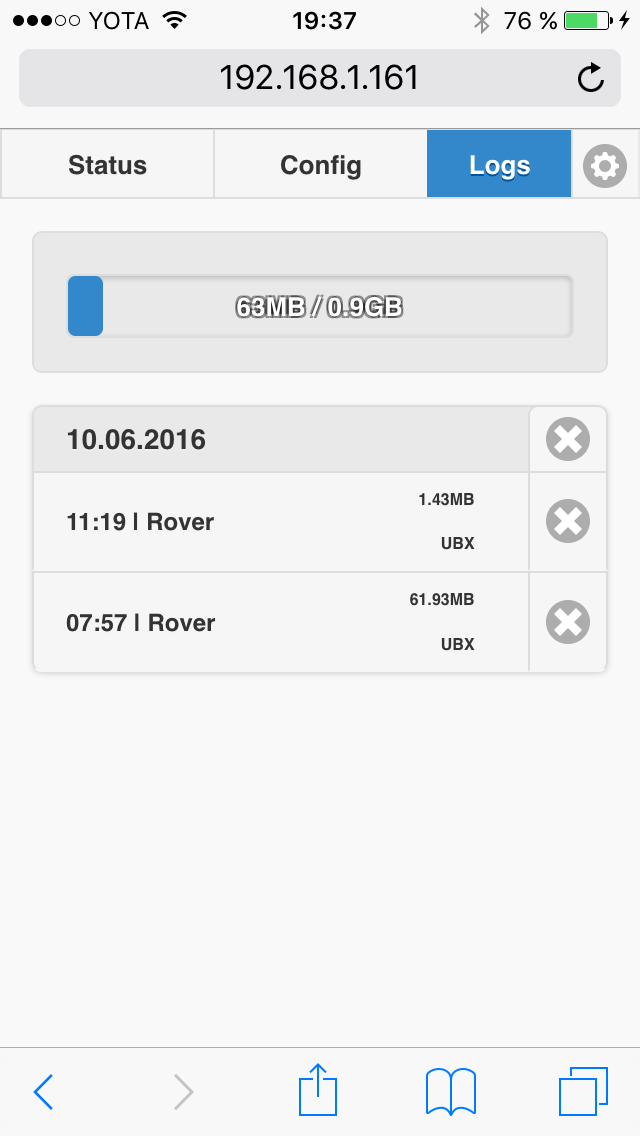
\includegraphics[width=.35\linewidth]{ui_testing_logs_tab}
    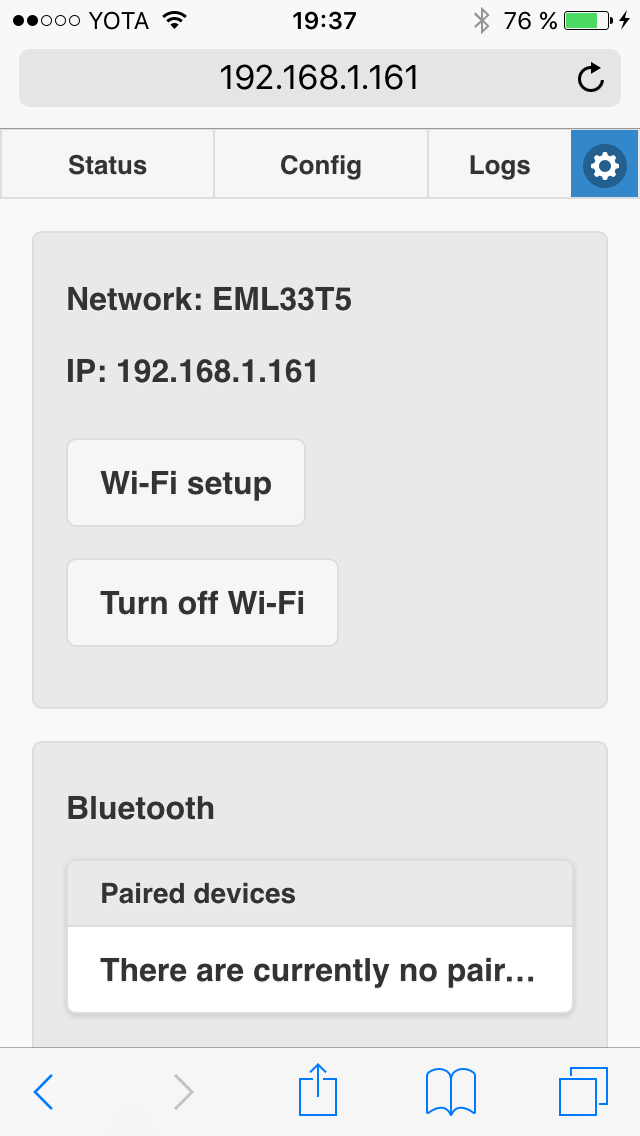
\includegraphics[width=.35\linewidth]{ui_testing_settings_tab}
    \caption{Logs и Settings}
  \end{subfigure}\par\medskip
  \caption{Вкладки приложения в браузере смартфона}
\end{figure}

\clearpage

\subsection{Тестирование работы режима ровера} \label{subsect4_2_2}

\underline{Исходные данные.} Приложение запущено и веб-страница открыта в браузере.

\underline{Ожидаемый результат.} При старте в режиме ровера во вкладке \textbf{Status} отображаемый режим работы должен измениться на \textbf{single}, а график должен показать уровни приема спутников, при условии наличии доступа к антенне на используемом приемнике. В логах, доступных при помощи \textbf{journalctl} должны отсутствовать ошибки.

\underline{Последовательность действий:}

\begin{enumerate}
  \item Перейти во вкладку \textbf{Config};
  \item Нажать на кнопку \textbf{Start};
\end{enumerate}

\underline{Результат.} Совпал с ожидаемым. На группе рисунков 4.2 представлены результаты старта режима ровера вместе с подключенной антенной.

\begin{figure}
  \label{img:latex}
  \center
  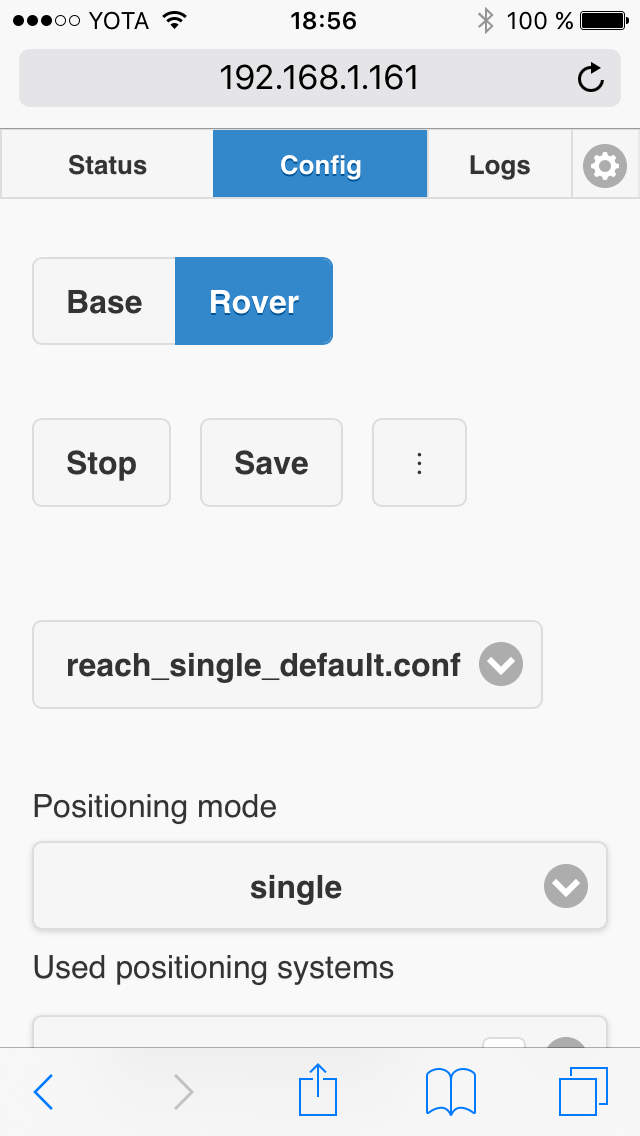
\includegraphics[width=.35\linewidth]{ui_testing_rover_start}
  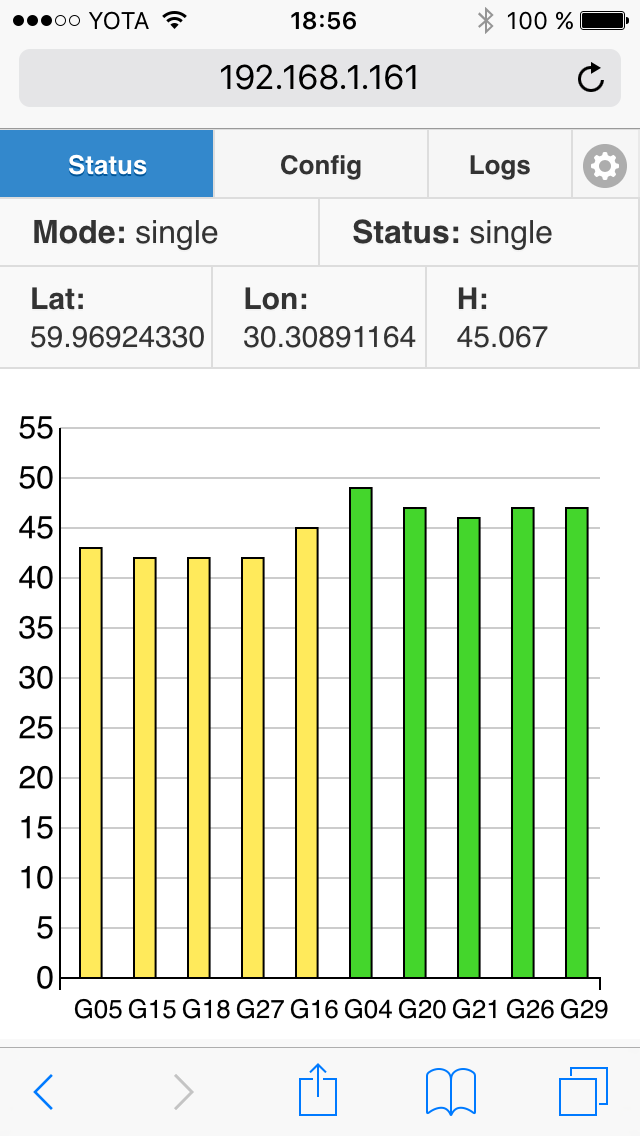
\includegraphics[width=.35\linewidth]{ui_testing_rover_started}
  \caption{Старт в режиме ровера и изменившийся экран статуса}
\end{figure}

\subsection{Тестирование конфигурации режима ровера} \label{subsect4_2_3}

\underline{Исходные данные.} Приложение запущено в режиме ровера.

\underline{Ожидаемый результат.} После настройки приема поправок с базы на графике отобразятся уровни приема спутников базы, а режим работы изменится на \textbf{kinematic}.

\begin{enumerate}
  \item Перейти во вкладку \textbf{Config} и изменить текущий режим работы на \textbf{kinematic};
  \item Указать источник поправок. В данном случае - база доступная в локальной сети;
  \item Hажать кнопку \textbf{Save} и подтвердить перезапуск с новыми параметрами.
\end{enumerate}

\underline{Результат.} Совпал с ожидаемым. На группе рисунков 4.3 представлен процесс настройки ровера, а на рисунке 4.4 - вкладка Status после успешной настройки.

\begin{figure}
  \label{img:latex}
  \center
  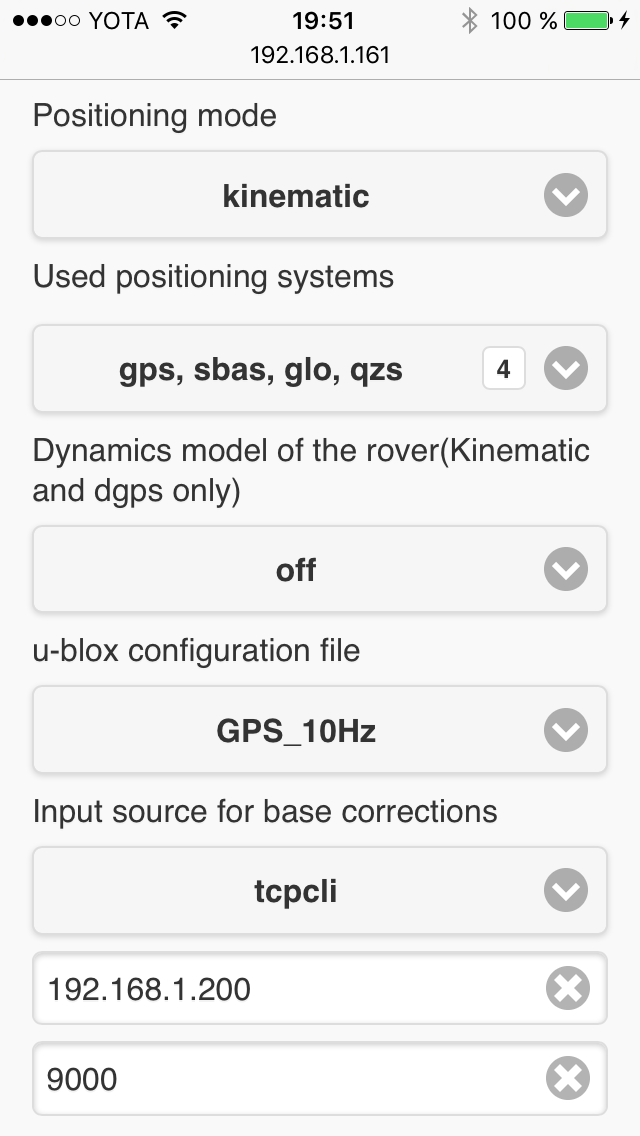
\includegraphics[width=.35\linewidth]{ui_testing_rover_settings}
  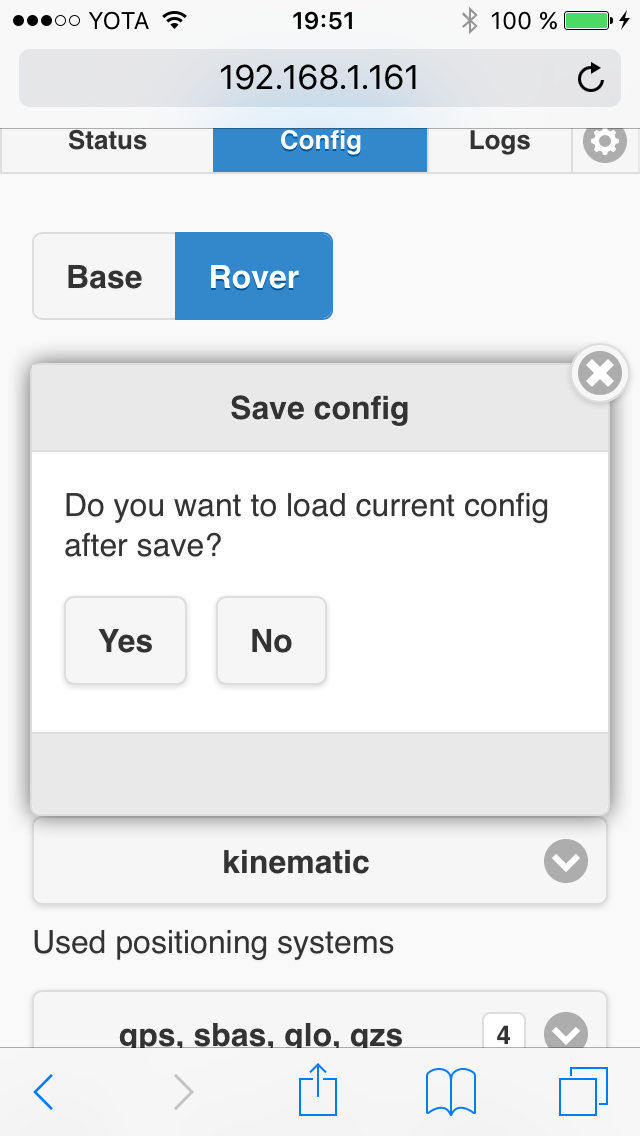
\includegraphics[width=.35\linewidth]{ui_testing_rover_load_settings}
  \caption{Настройка ровера  для приема поправок с базы}
\end{figure}

\begin{figure}[ht]
  \center
  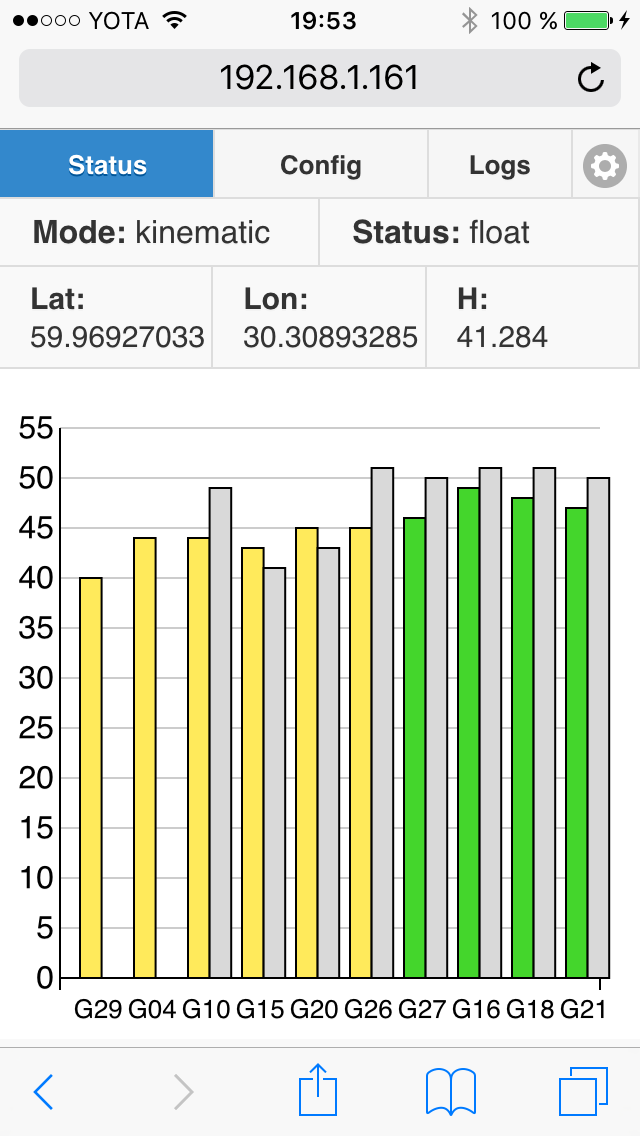
\includegraphics [scale=0.3] {ui_testing_rover_kinematic}
  \caption{Статус ровера при получении поправок с базы}
  \label{img:latex}
\end{figure}

\clearpage

\subsection{Запуск режима базы и проверка отправки поправок} \label{subsect4_2_3}

\underline{Исходные данные.} Приложение запущено в режиме ровера.

\underline{Ожидаемый результат.} Запущенный режим базы с поправками, доступными через TCP порт.

\underline{Последовательность действий.}

Каждое из действий изображено на группе рисунов 4.5.

\begin{enumerate}
  \item Перейти во вкладку \textbf{Config}, перейти в режим базы с помощью переключателя в верхней части вкладки;
  \item Настроить отправку поправок в TCP сокет;
  \item Запустить с помощью кнопки \textbf{Save \& Load};
\end{enumerate}

\begin{figure}
  \label{img:latex}
  \center
  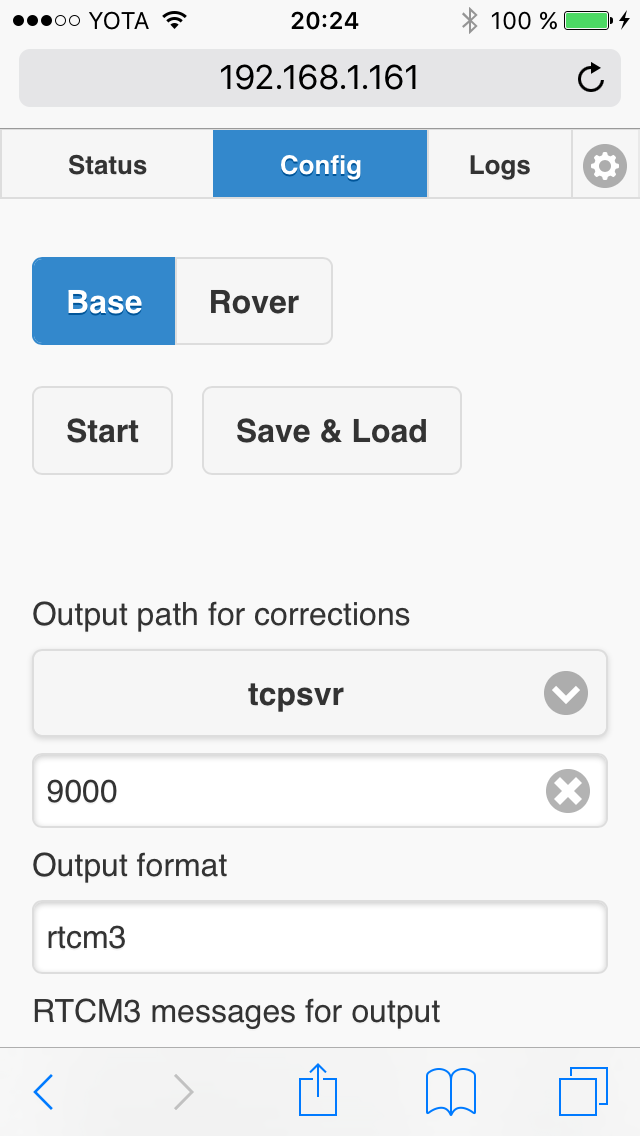
\includegraphics[width=.3\linewidth]{ui_testing_base_mode}
  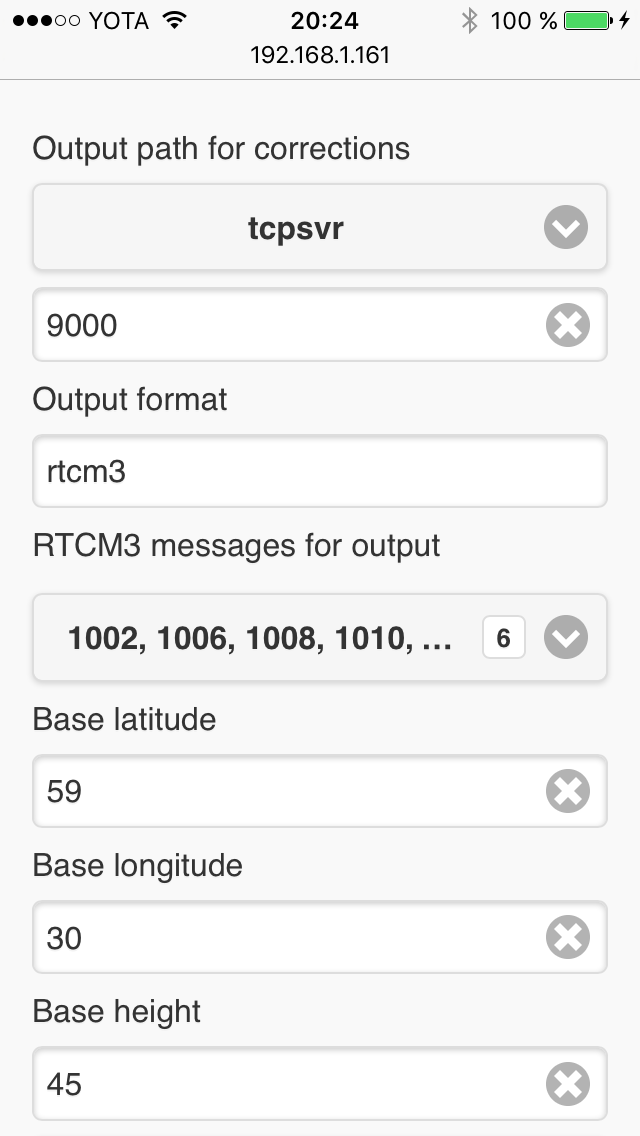
\includegraphics[width=.3\linewidth]{ui_testing_base_settings}
  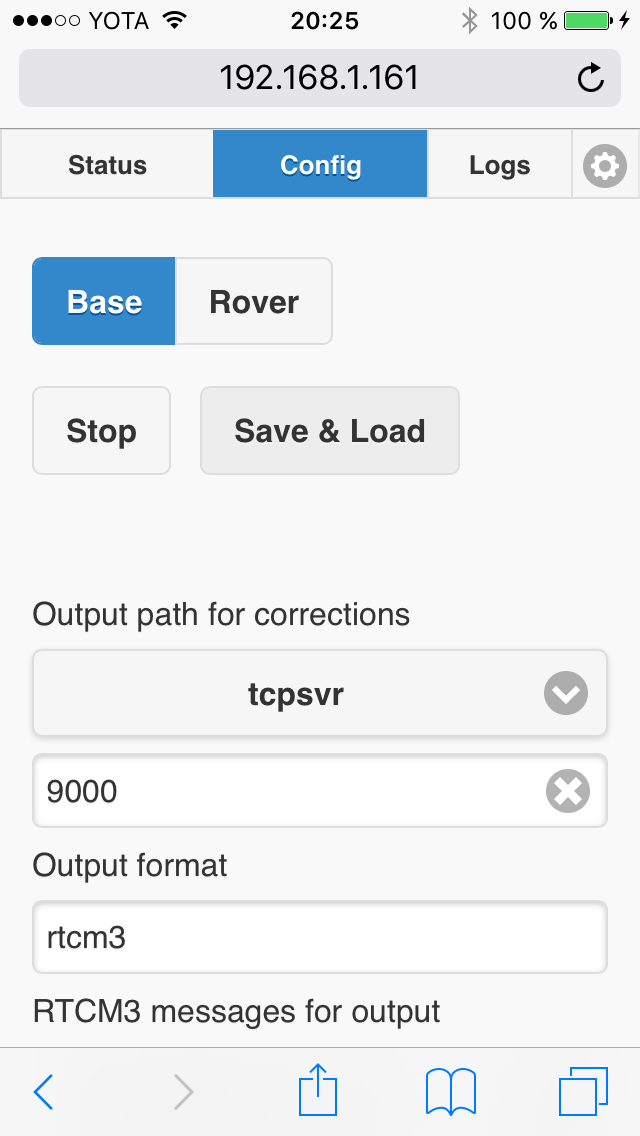
\includegraphics[width=.3\linewidth]{ui_testing_base_settings_load}
  \caption{Настройка режима базы}
\end{figure}

\underline{Результат.} Совпал с ожидаемым. Для проверки доступности поправок на TCP порту 9000 была использована программа \textbf{netcat}. Результат в виде бинарного RTCM3 протокола, который корректно не отображается в терминале, представлен на рисунке 4.6.

\clearpage

\begin{figure}[ht]
  \center
  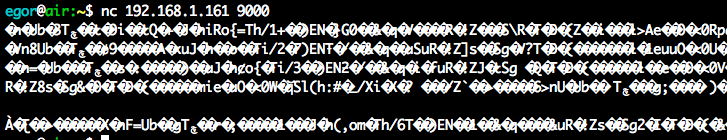
\includegraphics [scale=0.4] {ui_testing_base_corrections}
  \caption{Поправки, принятые с помощью netcat}
  \label{img:latex}
\end{figure}

\subsection{Тестирование скачивания и конвертирования логов} \label{subsect4_2_4}

\underline{Исходные данные.} Приложение запущено.

\underline{Ожидаемый результат.} Возможность скачать любой лог из списка, причем перед скачиванием он будет сконвертирован в формат RINEX.

\underline{Последовательность действий.}

Каждое из действий изображено на группе рисунов 4.6.

\begin{enumerate}
  \item Перейти во вкладку \textbf{Logs};
  \item Кликнуть на один из логов в представленном списке;
  \item Дождаться окончания таймера конвертации;
  \item Дождаться автоматического скачивания;
\end{enumerate}

\underline{Результат.} Совпал с ожидаемым. При клике на лог начался процесс конвертации, который не блокирует работу с приложением. По окончании обратного отсчета началось скачивание zip архива с RINEX логом и оригинальным логом в формате приемника.

\begin{figure}
  \label{img:latex}
  \center
  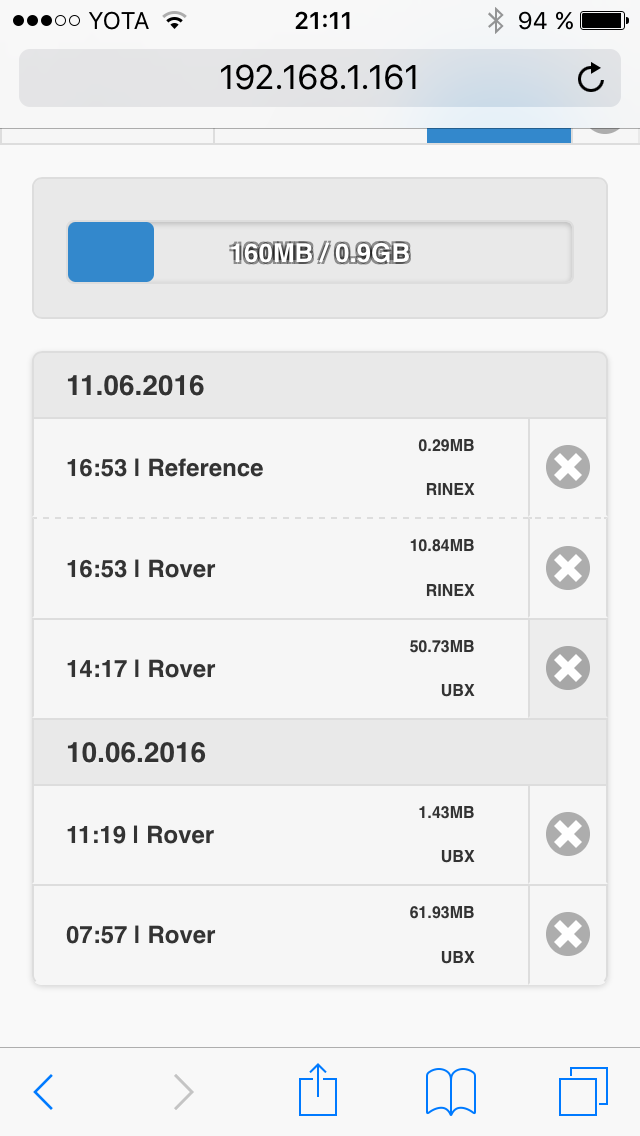
\includegraphics[width=.3\linewidth]{ui_testing_logs_list}
  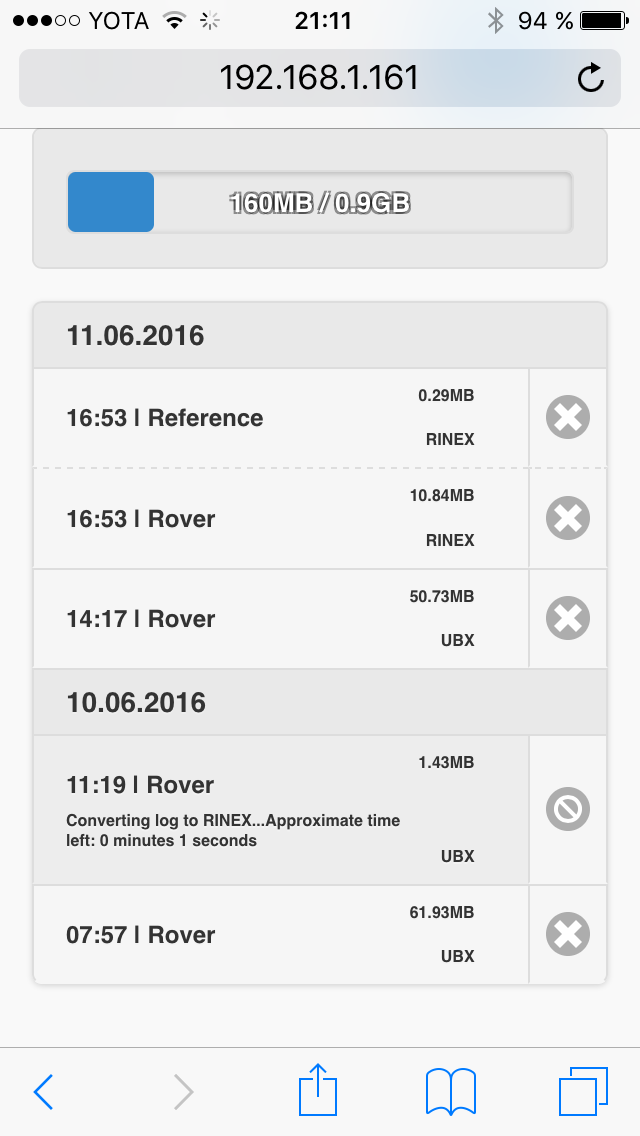
\includegraphics[width=.3\linewidth]{ui_testing_log_conversion}
  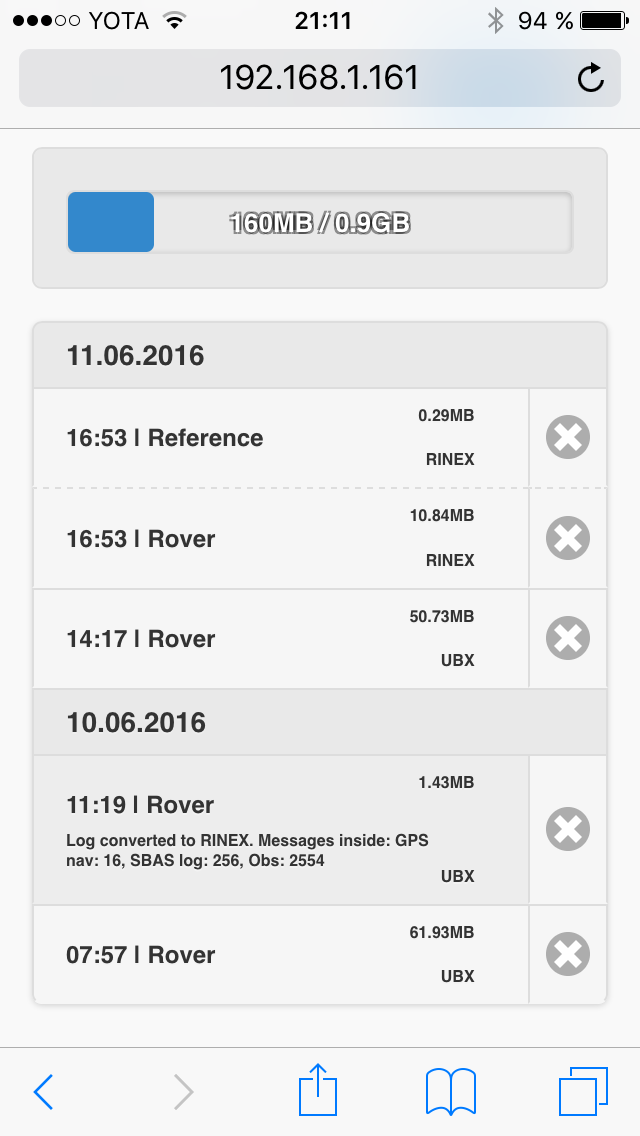
\includegraphics[width=.3\linewidth]{ui_testing_log_converted}
  \caption{Настройка режима базы}
\end{figure}


















